\documentclass{article} % For LaTeX2e
\usepackage{hyperref}
\usepackage{url}
\usepackage{amsmath}
\usepackage{amssymb}
\usepackage{bm}
\usepackage{pgf}
\usepackage{array}
%\documentstyle[nips14submit_09,times,art10]{article} % For LaTeX 2.09


\title{Experiments on learning to communicate}


\author{
Hugo Berard, Tom Bosc
}

% The \author macro works with any number of authors. There are two commands
% used to separate the names and addresses of multiple authors: \And and \AND.
%
% Using \And between authors leaves it to \LaTeX{} to determine where to break
% the lines. Using \AND forces a linebreak at that point. So, if \LaTeX{}
% puts 3 of 4 authors names on the first line, and the last on the second
% line, try using \AND instead of \And before the third author name.

\newcommand{\fix}{\marginpar{FIX}}
\newcommand{\new}{\marginpar{NEW}}
\DeclareMathOperator*{\argmin}{\arg\!\min}
\DeclareMathOperator*{\argmax}{\arg\!\max}
\DeclareMathOperator{\E}{\mathbb{E}}

\usepackage{natbib}
\begin{document}

\maketitle

\section{Introduction}
There is a recent surge of papers on the theme of learning to communicate \cite{sukhbaatar2016learning} \cite{foerster2016learning} \cite{lazaridou2016multi} \cite{mordatch2017emergence}. The common setting is a Partially Observable Markov Decision Process (POMDP) where several agents act at each timestep and share the same rewards. The environments are designed so that communication is necessary to for agents to get a reward: one agent has an information which another agent needs to pick the action that leads to the rewards. The emphasis is on learning the language, that is, tokens emitted by agents don't have a predetermined meaning. Rather, the meaning emerges from its use. 

The goal of this project is to study how Policy Gradients (PG) methods and Deep Q-Learning (DQN) perform in this kind of POMDP with several agents. The evaluation of the method is done on a grid world where communication is necessary to maximize the returns. 

\section{Models}
\subsection{Recurrent Policy Gradients}
Indirect reinforcement learning approaches to control require learning a state-action value function $Q(s,a)$. Policy are derived from $Q$ by maximizing over actions (\textit{greedifying}). On the contrary, with Policy Gradient (PG) methods, the policy is directly parametrized. There are several motivations for doing that\cite{sutton1998reinforcement}. Firstly, in control problems, the $Q$ function is not the quantity of interest. Furthermore, computing this quantity can be a harder problem. Finally, by comparison with $\epsilon$-greedy policy where the entropy or randomness of the policy is fixed using $\epsilon$, here it is flexible and adjusted during the learning process. Here we consider learning stochastic policies. The policy is denoted by $\pi_{\theta}$ and the objective is then to find the parameters $\theta$ that maximize the value function of the policy evaluated in the start state:
$$
argmax_{\theta} v_{\pi_{\theta}}(s_0)
$$

PG methods require computing the gradient, or at least estimating it when the policy is not differentiable. The policy gradient theorem states that:
$$
\nabla_{\theta} v_{\pi_{\theta}} = \sum_s d_{\pi_{\theta}} \sum_a \nabla \pi_{\theta}(a|s) q_{\pi_{\theta}}(s,a) % = E_{\pi_{\theta}}[\sum_a \gamma^t \nabla \pi(a|S_t) q_{\pi}(S_t,a)]
$$

This sum over states and actions is actually an expectation under the policy $\pi_{\theta}$ and the environment's dynamics:
$$
\nabla_{\theta} v_{\pi_{\theta}} = E_{\pi_{\theta}}[\gamma^t R_t \nabla log \pi_{\theta}(A_t|S_t)] % = E_{\pi_{\theta}}[\sum_a \gamma^t \nabla \pi(a|S_t) q_{\pi}(S_t,a)]
$$

We can estimate the empirical return with Monte-Carlo and the log of the policy is known so this estimate is tractable.

%$$
%\nabla_{\theta} E_{\pi_{\theta}}[R_t] = E[\frac{\partial \pi}{\partial y}] \frac{\partial y}{\partial \theta}
%$$

In POMDPs, the agent has to infer the state its in. Indeed, it only has access to an observation which is a function of the state. This partial observability is generally dealt with by adding memory to the agent: at each timestep, the agent updates its memory which contains probabilities to be in the true states. Based on this probability that we call belief\footnote{Because of the equivalence between POMDPs and Belief MDPs, which are MDPs where the states live in the probability simplex on the states of the original POMDP.}, the agent can decide on actions. 

Recurrent Policy Gradients\cite{wierstra2010recurrent} (RPG) is a PG algorithm that can solve POMDPs. It combines REINFORCE with Recurrent Neural Networks (RNN). REINFORCE can be used jointly with backpropagation as it is in general a gradient estimator\cite{williams1992simple}. If the policy $\pi$ is a probability mass or density function parametrized by parameters $y(\theta)$ where $y$ is a deterministic function, we can decompose the expectation of the gradient using the chain rule:

$$ E[\frac{\partial \pi}{\partial \theta_i}] = E[\frac{\partial \pi}{\partial y}] \frac{\partial y}{\partial \theta_{i}} $$

In the case of RPG, REINFORCE is computed on the stochastic outputs units of the RNN (first factor of RHS) whereas regular backpropagation is used on the deterministic part of the RNN (second factor of RHS). Here, $y_t = f(h_t, \theta)$ where $h_t$ is the hidden state of the LSTM at timestep $t$. The hidden state can be seen as the belief and the updates are learned and represented as the transition matrix. The inputs of the LSTM are the observations of the agent, the last action that was performed by the agent (necessary because the policy is stochastic) and the reward. The outputs of the LSTM are the parameters of the distribution from which the actions will be sampled.

A Long Short-Term Memory\cite{hochreiter1997long} (LSTM) RNN is chosen for convenience and performance. 

To reduce variance, a baseline is used. In MDPs, baselines are taken to be $v_{\pi}$ so that the log gradient term is weighted by the advantage function $q_{\pi}(s,a) - v_{\pi}(s) = A_{\pi}(s,a)$. Since we are in a POMDP, we can't estimate the state value function but instead learn an approximation based on the belief state. It is recommended to use another RNN as a baseline which takes the same inputs (except for the reward) and produce an estimate of the empirical returns. We can train this RNN supervisedly as we have access to the empirical returns.

The learning process is done offline. By storing histories like DQN's experience replay, we can use minibatches that further reduce the variance of our gradient estimates as their sizes grow.

\subsection{Recurrent Deep-Q-Learning}
When dealing with a large state space tabular representation becomes impractical to use. To remedy to this problem we can use function approximation and parametrize the Q-value function as a function of the state. Recently it has been shown \cite{mnih2015human} empirically that despite not having any convergence guarantee, neural networks performs well.
The parameters are updated following the usual subgradient of the MSE between the predicted Q-value and the target:

$$\theta_{t+1} = \theta_t + \alpha(r+\max_a Q_{\hat{\theta}}(s_{t+1}, a) - Q_{\theta_t}(s_t, a_t))\nabla_{\theta_t}Q_{\theta_t}(s_t, a_t)$$

In order to work well, we need to introce several tricks:

\textbf{Replay Memory}: Instead of updating online, the transitions are stored in a replay memory, and at each time step a batch of transitions is sampled from the memory to train the model.

\textbf{Target Network}: When computing the target, the Q-value for the next-step, we use a copy of the network but with a set of parameters $\hat{\theta}$ only updated every $n$ iterations.


\textbf{Recurrent Network}: To deal with the fact that the environement is partially observable, we add a recurrent layer so that the agent is able to remember the previous observation. To train the model, following \cite{hausknecht2015deep} we sample random episodes from the replay memory and unroll the episode for $n$ steps.

\section{Gridworld experiment}
This experiment is a simplified variant of \cite{mordatch2017emergence}. The main difference is that our environment has discrete action space and state space. This allows for a fairer comparison between RDQN and RPG. Indeed, Q-learning updates are computed by maximizing the action-state value function $Q(s,a)$ over actions which is in general costly in continuous action space. 

The environment is a POMDP. There are $N$ agents and $M$ landmarks which are defined by an integer $i$ and their respective coordinates $x_i$ on a squared grid. At each timestep, agents choose an action from $A={left, right, up, down}$ which makes them move\footnote{For simplicity's sake, we allow several agents to be on the same landmark at the same time.}. Agents know their own position as well as positions of the landmarks. In addition, each agent $i$ observes its own goal $g_i$ which is to direct another agent to one of the landmarks. All the agents are rewarded at once every first timestep one agent reach its assigned landmark. Because of partial observability of goals, agents need to communicate the location of the goal landmark to the goal agent. For that purpose, we allow the agent to emit one token $c \in C = \{1..V\}$ at each timestep which will be visible at the next timestep to everyone. Technically, the action space is now $C \times A$.

To sum up, at each timestep, the observation of agent $i$ is a vector $o_i(t) = [i, x_i, c_{1..N}, g_i]$

The fact that the rewards are shared is essential. Without this, agents would have no incentive to make other agents fulfill their goals.

\section{Results}
For all experiments we use Adam \cite{kingma2014adam} with $alpha=1.10^{-3}, \beta_1=0.9, \beta_2=0.999$ and minibatches of size 32. During training we follow an $\epsilon$-greedy policy starting with $1$ and decaying lienarly to $0.1$ over $5.10^4$ steps. We used a replay memory of 25 000 transitions and the target network was updated every 10 000 updates.
\subsection{RPG}
Work in progress. It is still computing, should be finished by saturday 22 before midday.
\subsection{2 Agents Fully Observable}
To test the environement and the approach we first train 2 agents, on a fully observable task with 2 landmarks.
We tried both using a recurrent layer and without. The architecture used  consist of one hidden layer of 32 units, followed by a layer that output one single value per action corresponding to the Q-value of that function. For the recurrent architecture, the hiddent layer is replaced by a lstm layer with the same number of units, and the episode was unrolled for 4 time steps.

For both models the training is quite unstable, and starts to diverge as soon as the optimal policy is almost reached. We're not sure why this behavior occur, we tried to anneal the learning rate but it doesn't seem to work better.

\begin{figure}[h]
\centering
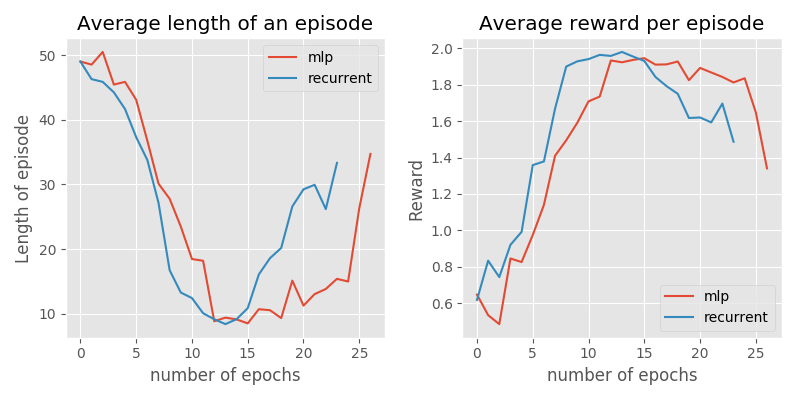
\includegraphics[width=\textwidth]{multiagent_mdp_results.png}
\caption{The average length and reward of the different models. The results are averaged over 100 episodes.}
\end{figure}

\subsection{2 Agents Partially Observable}
Unfortunately we were unable to make DQN works on that example.

\bibliographystyle{unsrt}  
\bibliography{bibliography}
\end{document}
